\section{Research}\label{sec:proposal}
\begin{frame}{Research}
	\begin{itemize}
		\setlength{\itemsep}{1em}
		\item<1-> This work is based on two premises:
		
		\begin{enumerate}[(i)]
			\setlength{\itemsep}{1em}
			\item<1-> that sensitive applications communicate over the NoC in MPSoCs, and are therefore vulnerable to interference by malicious applications; and
			
			\item<1-> that protection from software attacks is achieved by communication level protection; e.g., by defining safe communication paths for sensitive applications
		\end{enumerate}
		
		\item<1-> Therefore, a routing algorithm that is capable of defining safe routing paths for sensitive applications should enhance the overall system protection
	\end{itemize}
\end{frame}

%%%%%%%%%%%%%%%%%%%%%%%%%%%%%%%%%%%%%%%%%%
%%% THREAT MODEL %%%%%%%%%%%%%%%%%%%%%%%%%
%%%%%%%%%%%%%%%%%%%%%%%%%%%%%%%%%%%%%%%%%%
\subsection{Threat Model}
\begin{frame}{Threat Model}
	\begin{center}
		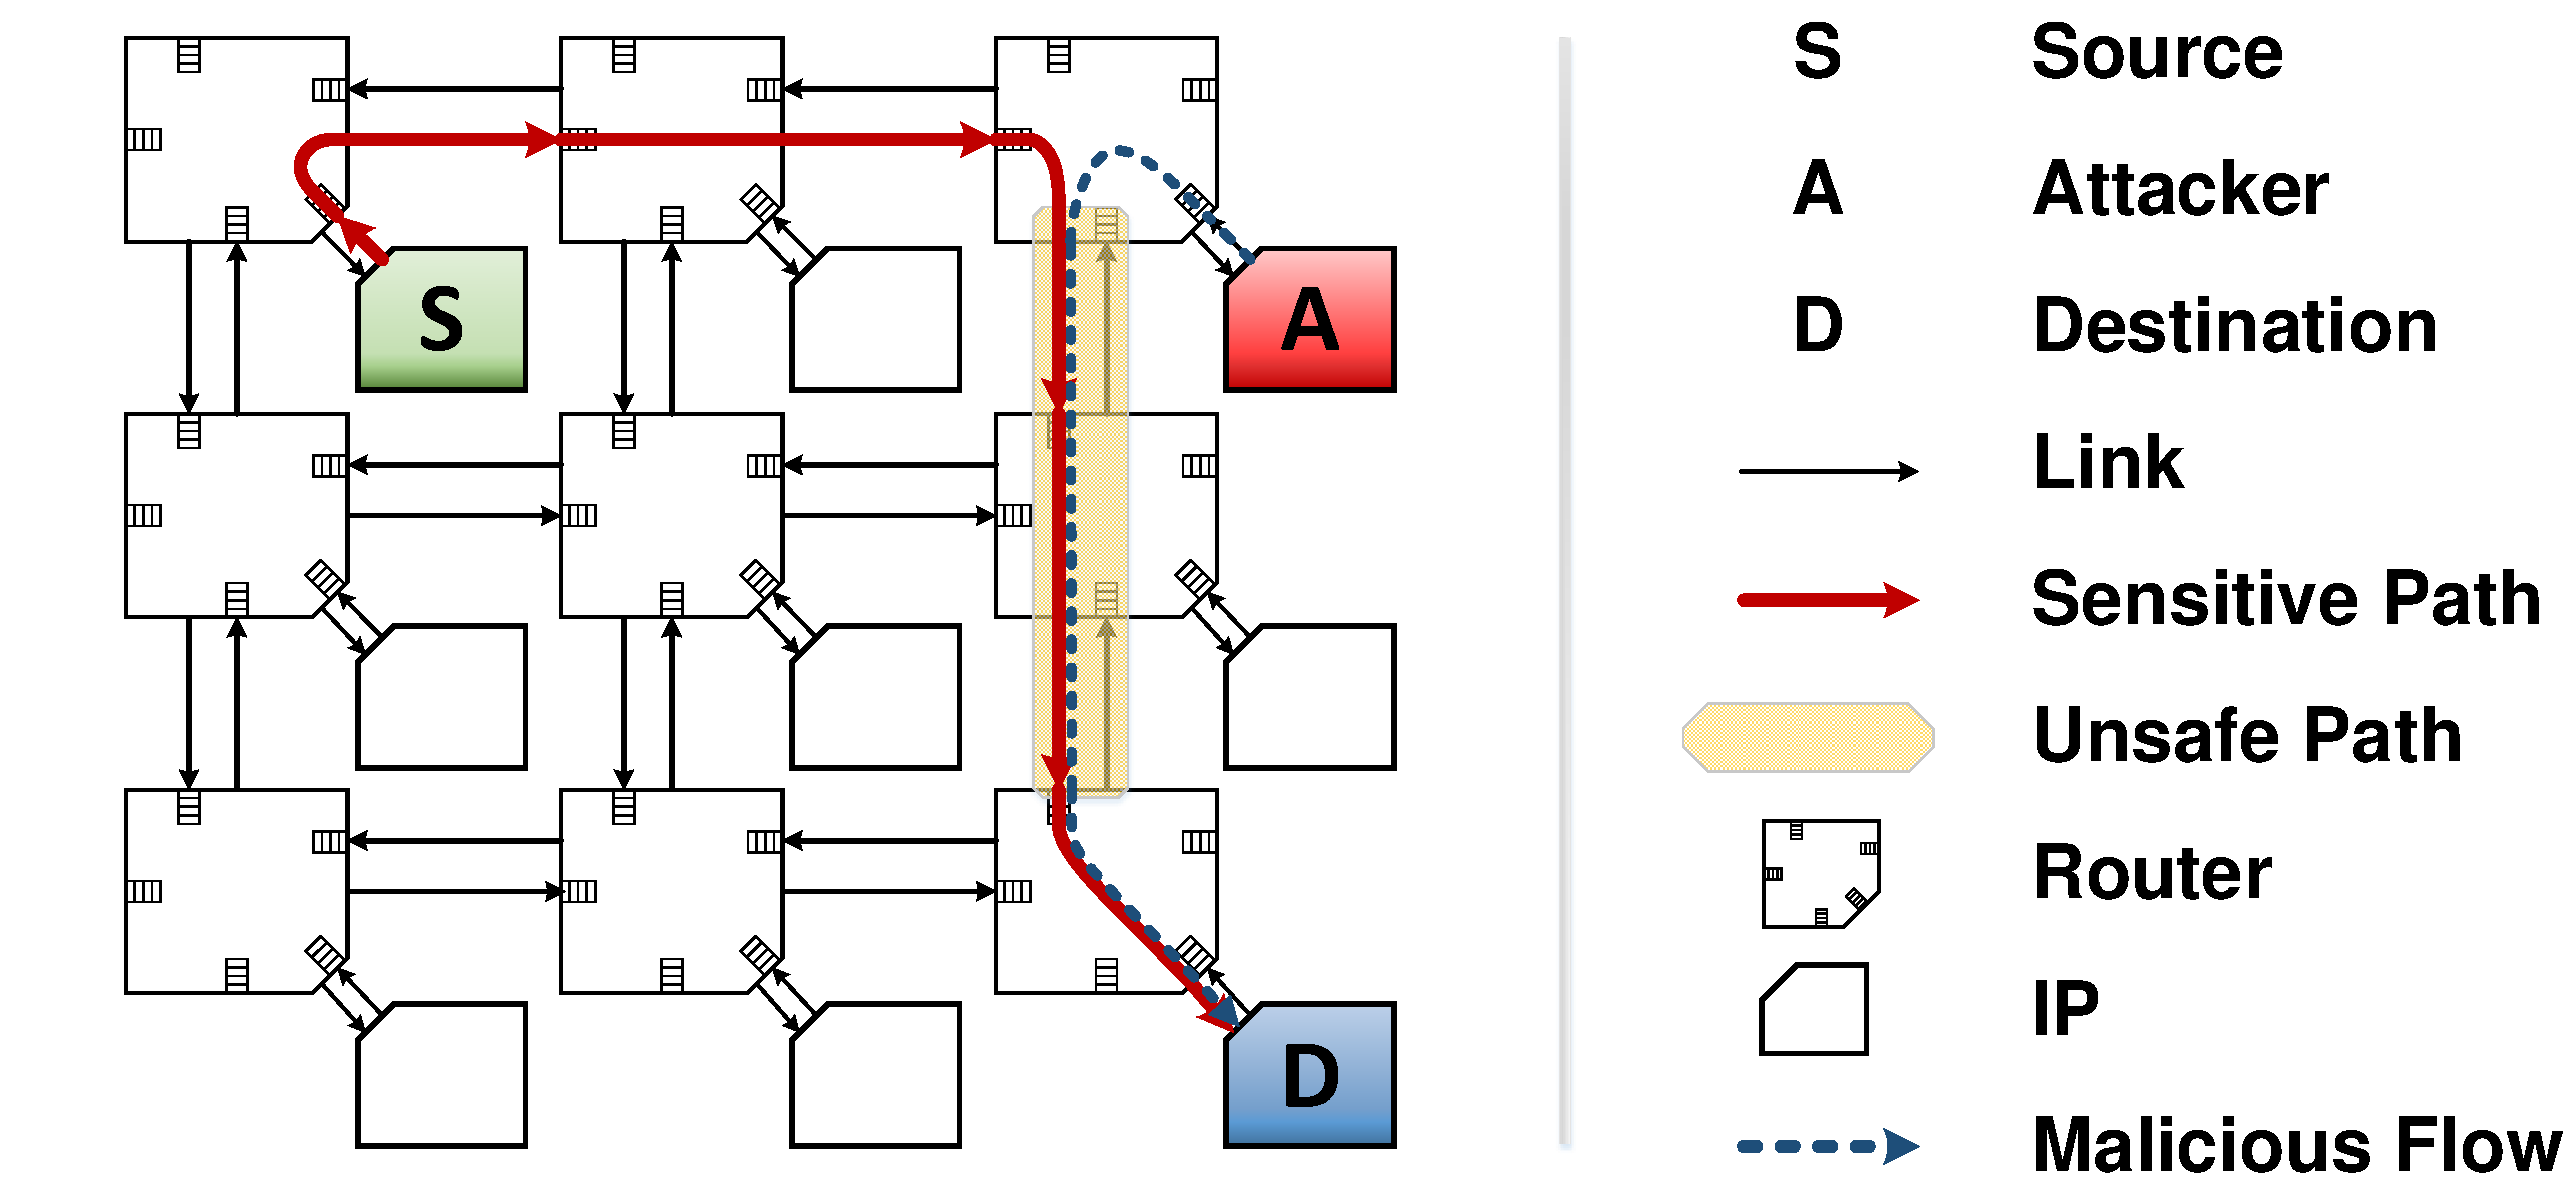
\includegraphics[width=0.75\linewidth]{images/threat_model/timing-attack.pdf}
	\end{center}
	\begin{itemize}
		\item<only@1> The NoC is considered secure, meaning that an attacker cannot tamper its resources
		
		\item<only@1> An attacker, aware of the sensitive path, can disrupt communication between a source and a destination
		
		\item<only@1> We consider that an attacker can either generate a \emph{DoS} or \emph{Timing Attack} on the sensitive path
	\end{itemize}
\end{frame}

%%%%%%%%%%%%%%%%%%%%%%%%%%%%%%%%%%%%%%%%%%
%%% SECURITY AWARE ROUTING %%%%%%%%%%%%%%%
%%%%%%%%%%%%%%%%%%%%%%%%%%%%%%%%%%%%%%%%%%
\subsection{Security Aware Routing}
\begin{frame}{Security Zones}
	\begin{center}
		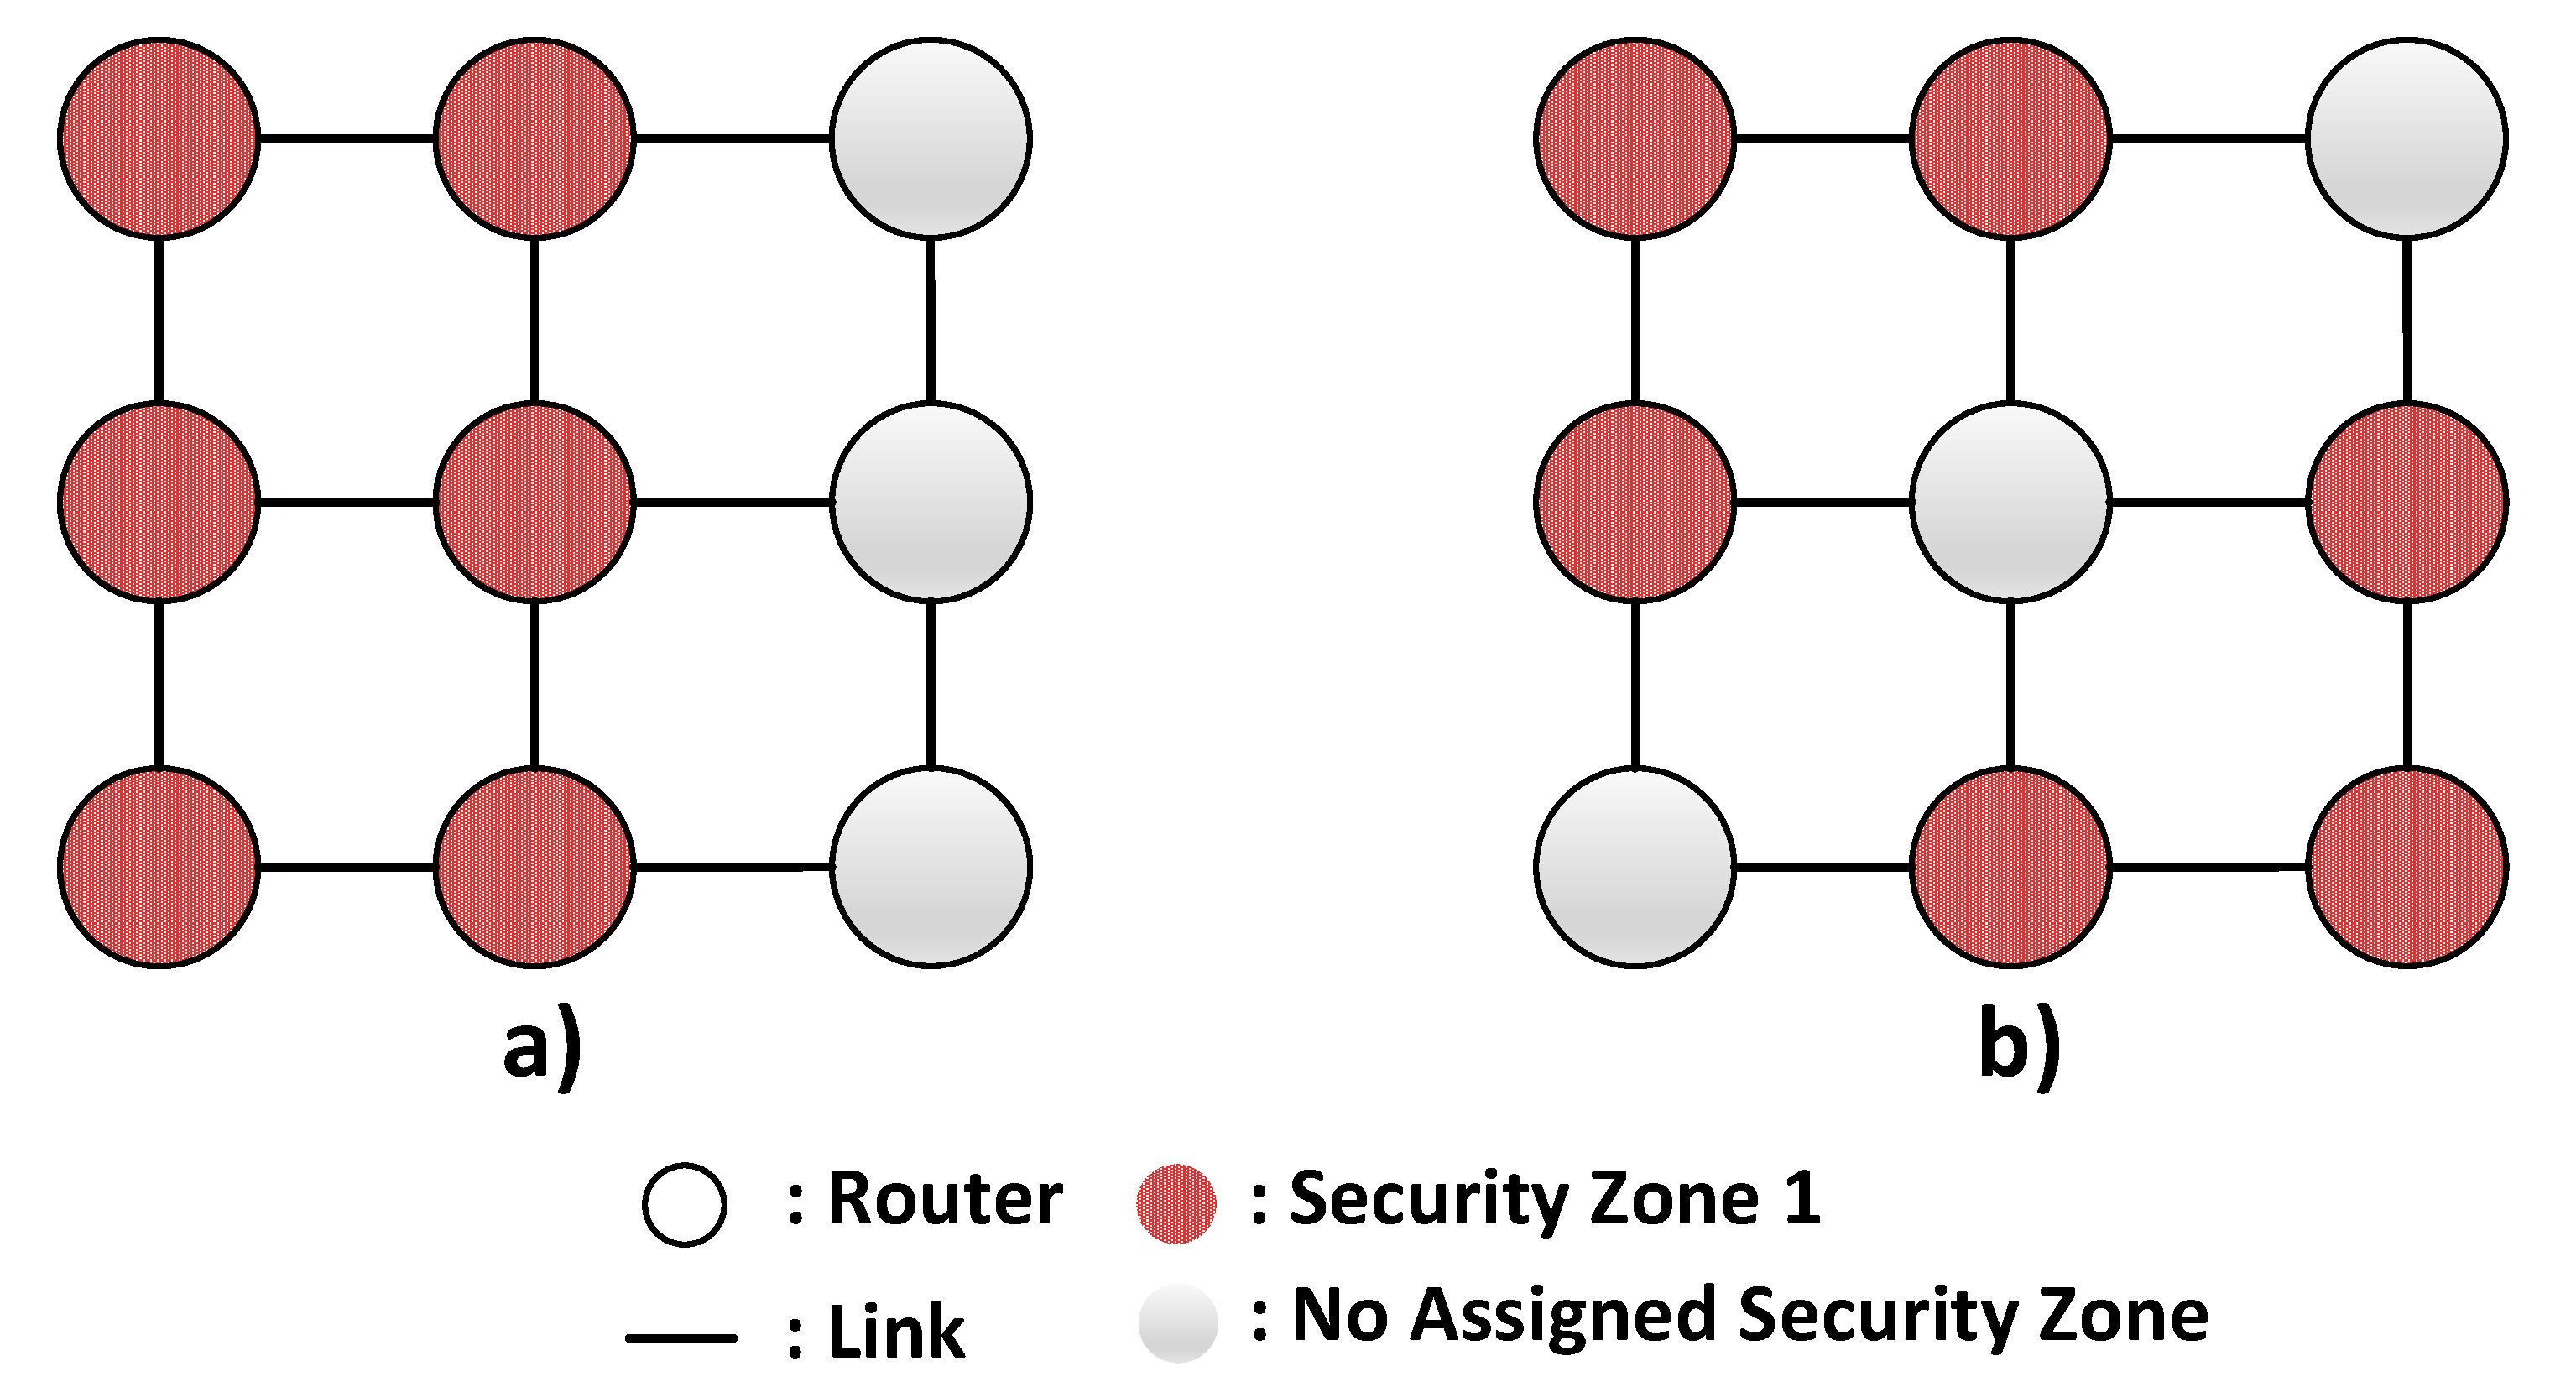
\includegraphics[width=0.60\linewidth]{images/secure_routing/security-zones-shapes.pdf}
	\end{center}
	\begin{itemize}
		\item<only@1> A security zone is a physical space (continuous or disrupted) that wraps IPs that execute critical applications
		
		\item<only@1> The task mapping of critical applications defines the shape of the security zone
		
		\item<only@1> Certain IP blocks might not be assigned to any security zone, e.g., idle resources or shared memories
	\end{itemize}
\end{frame}
\begin{frame}[t]{Communication in Security Zones}
	\begin{onlyenv}<1-3>
		\begin{center}
			\includegraphics<1>[width=0.85\linewidth]{images/secure_routing/security-zones-fiz.pdf}
			\includegraphics<2>[width=0.85\linewidth]{images/secure_routing/security-zones-piz.pdf}
			\includegraphics<3>[width=0.85\linewidth]{images/secure_routing/security-zones-iz.pdf}
		\end{center}
	\end{onlyenv}
	\begin{itemize}
		\item<only@1> \textit{\textbf{Full intra-zone communication (FIZ)}}: \emph{S} and \emph{D} are in the same $SZ$. The sensitive path is \textbf{completely} inside the $SZ$, e.g., the path from \emph{IP1} to \emph{IP2}
		
		\item<only@2> \textbf{\textit{Partial intra-zone communication (PIZ)}}: \emph{S} and \emph{D} are in the same $SZ$. However, the sensitive path is \textbf{partially} inside the $SZ$. , e.g., the path from \emph{IP3} to \emph{IP4}
		
		\item<only@3> \textbf{\textit{Inter-zone communication (IZ)}}: \emph{S} and \emph{D} are in different $SZ$, e.g., the path from \emph{IP5} to \emph{IP6}
	\end{itemize}
\end{frame}

\begin{frame}[t]{Segment-based Routing (SBR) - Deadlock Prevention}
	\begin{center}
		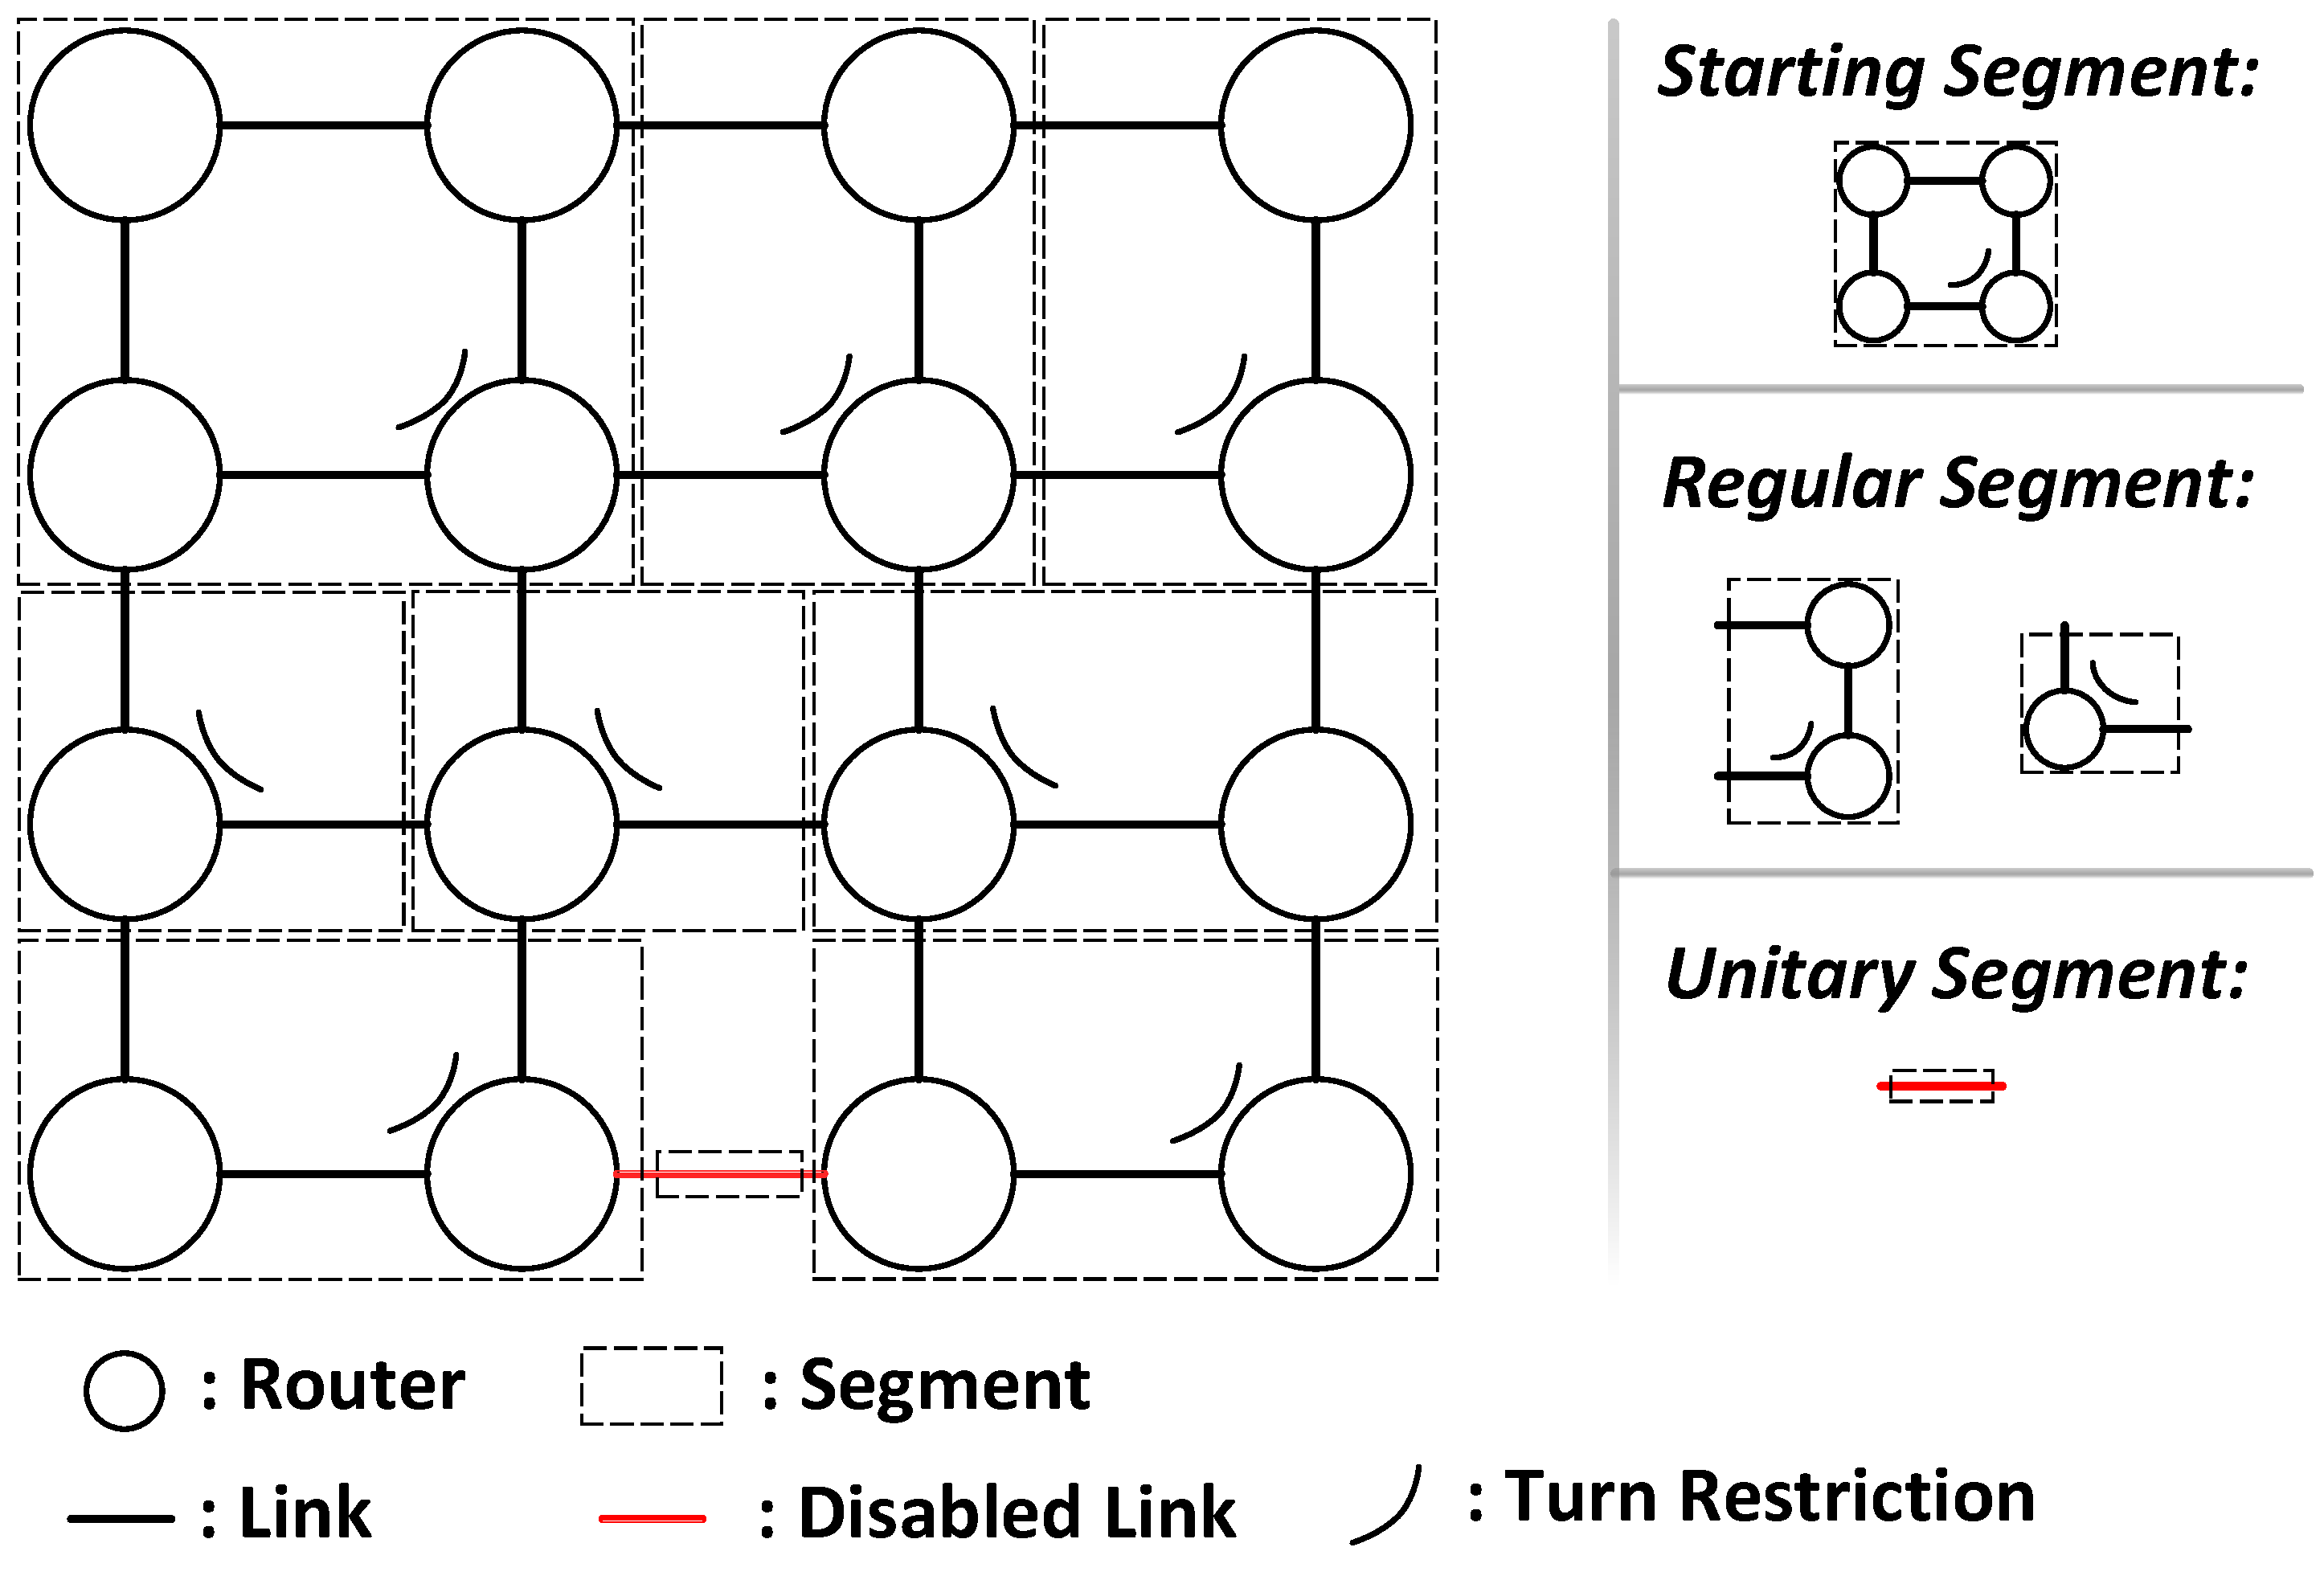
\includegraphics[width=0.65\linewidth]{images/secure_routing/sbr.pdf}
	\end{center}
	\begin{itemize}
		\item<only@+> Logically partitions the NoC into segments
		
		\item<only@+> Each segment contains a localized bidirectional turn restriction
		
		\item<only@+> Guarantees global deadlock freedom and reachability (as long as the NoC is connected)
	\end{itemize}
\end{frame}

\begin{frame}[t]{SBR-Security Zone Awareness (SBR-SZA)}
	\begin{onlyenv}<1-2>
		\begin{center}
			\includegraphics<1>[width=0.85\linewidth]{images/secure_routing/sbr-configs.pdf}
			\includegraphics<2>[width=0.75\linewidth]{images/secure_routing/sbr-sza.pdf}
		\end{center}
	\end{onlyenv}
	\begin{itemize}
		\item<only@1> Traditional SBR might place turn restrictions that causes \textbf{\textit{PIZ}} routing
		\item<only@2> SBR-SZA aims to create segments that tailor to security zone shapes
	\end{itemize}
\end{frame}

\begin{frame}{Region-based Routing (RBR) - Routing Algorithm}
	\begin{itemize}
		\setlength{\itemsep}{1em}
		\item<1-> Populates the routing tables of NoC routers, considering the turn restrictions of SBR
		
		\item<1-> Groups routing entries to greatly reduce table size (interval routing and port/destination sets)
		
		\item<1-> There are three steps in RBR computation:
		\begin{itemize}[i]
			\setlength{\itemsep}{0.5em}
			\item<1-> \textit{Routing Computation}: computes all source and destination pairs
			
			\item<1-> \textit{Region Computation}: joins entries based on input and output ports
			
			\item<1-> \textit{Region Merge}: merges overlapping regions to reduce routing entries
		\end{itemize}
	\end{itemize}
\end{frame}

%%%%%%%%%%%%%%%%%%%%%%%%%%%%%%%%%%%%%%%%%%
%%% MODELING %%%%%%%%%%%%%%%%%%%%%%%%%%%%%
%%%%%%%%%%%%%%%%%%%%%%%%%%%%%%%%%%%%%%%%%%
\subsection{Modeling}
\begin{frame}[t]{Modeling}
	\begin{center}
		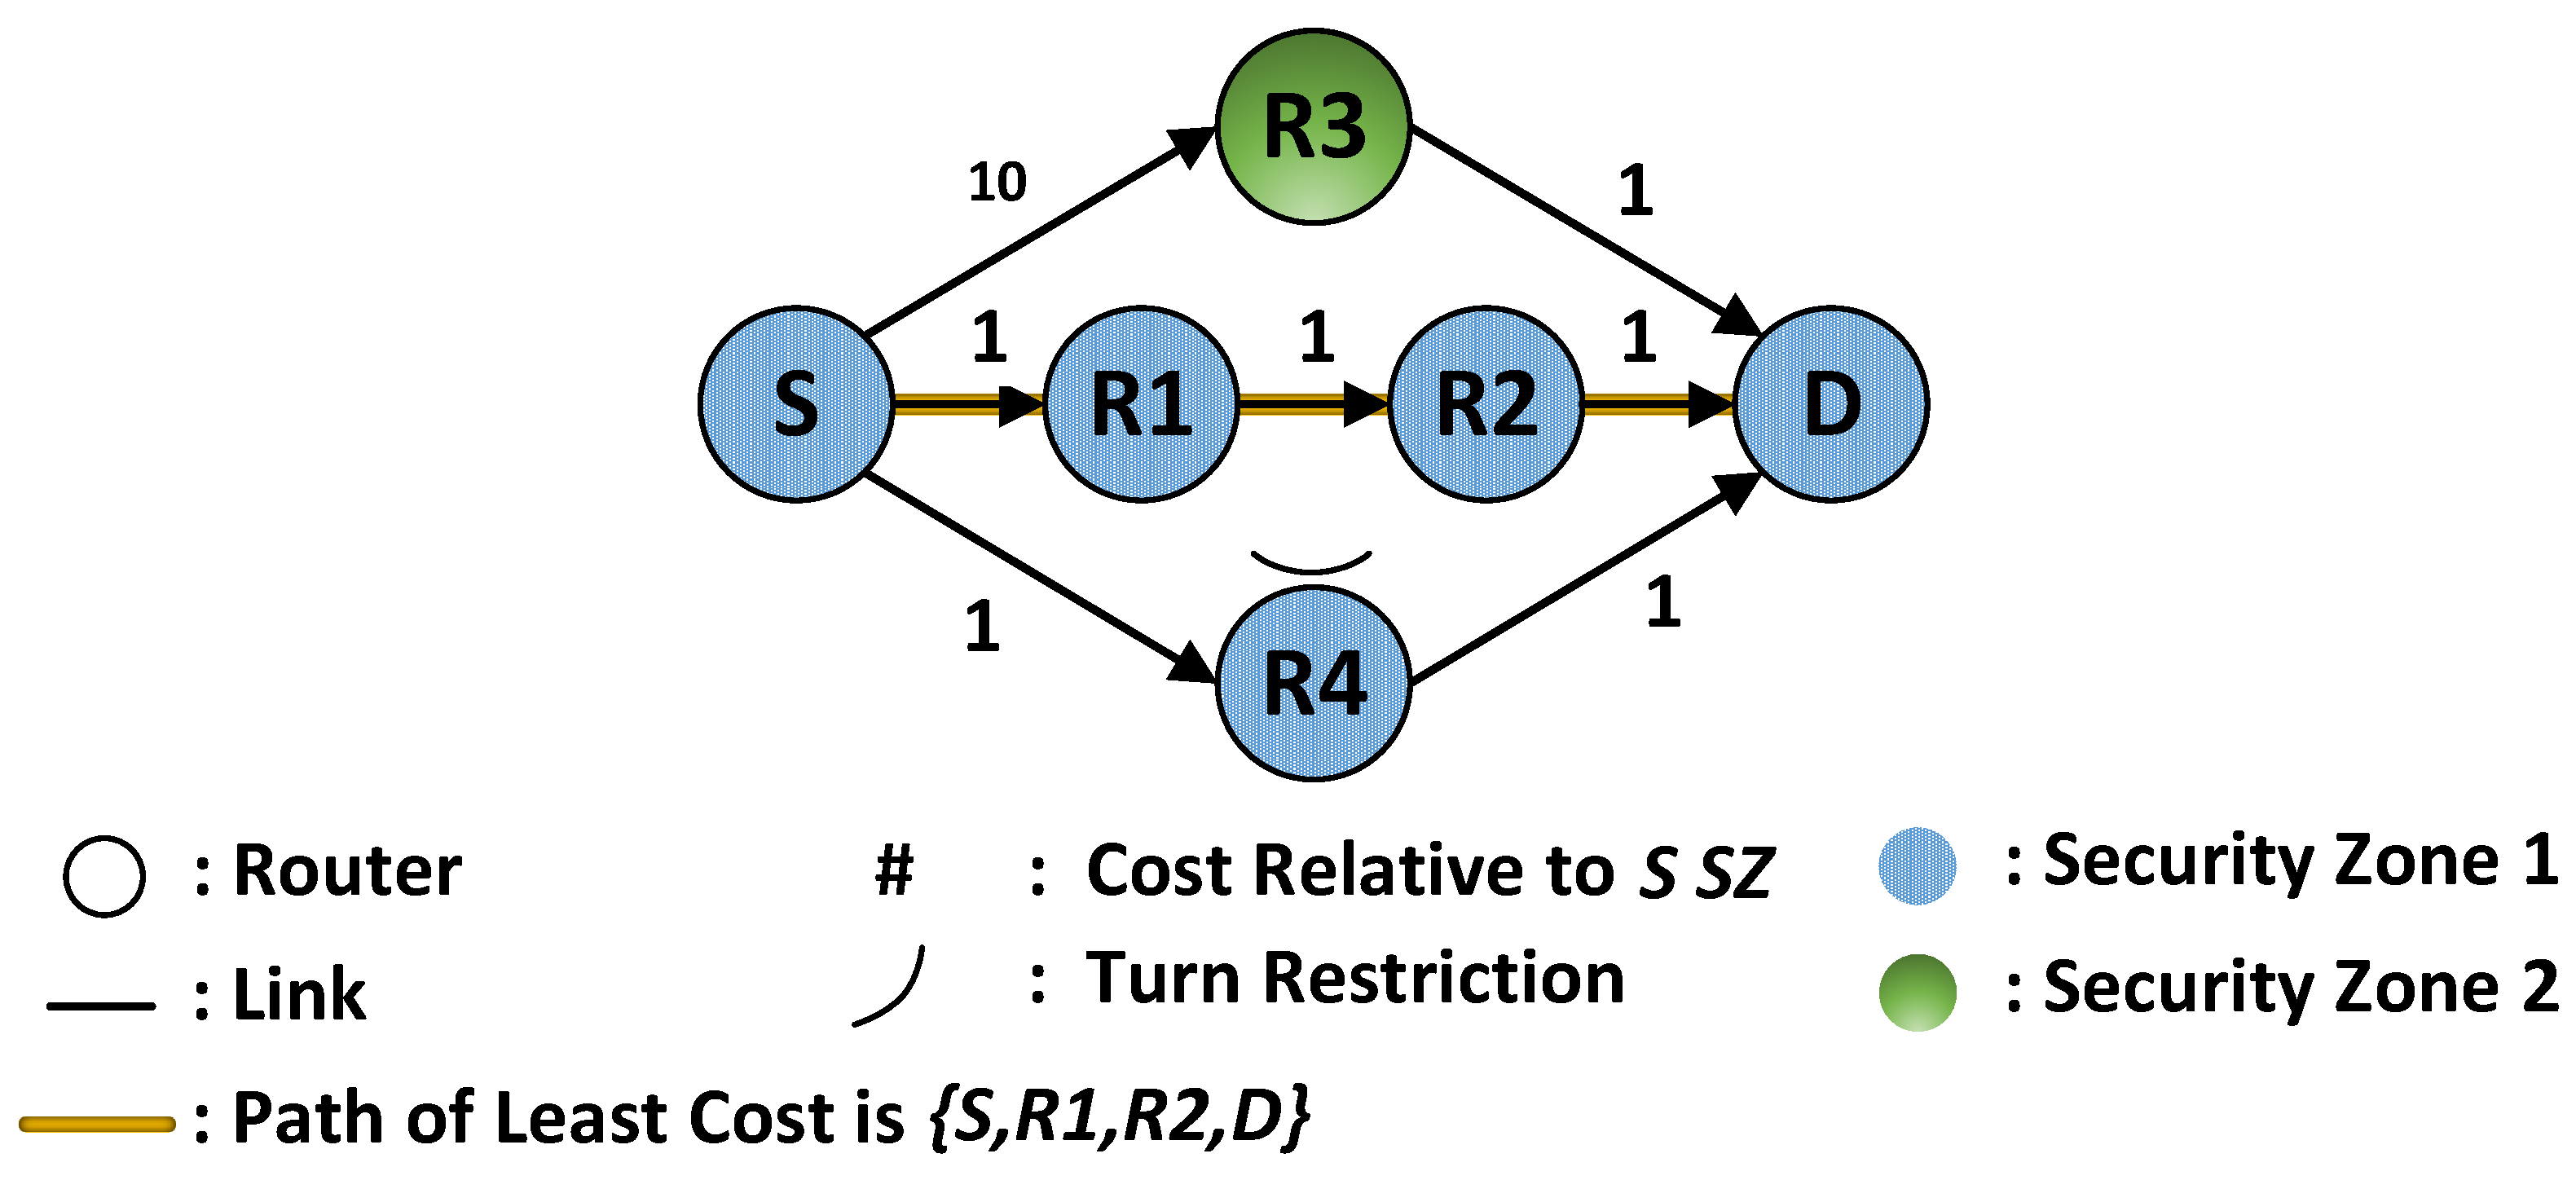
\includegraphics[width=0.75\linewidth]{images/secure_routing/rbr-path-finding.pdf}
	\end{center}
	\begin{itemize}
		\item<only@1> The NoC is modeled as a graph, with IP/Routers as vertices and links as edges
		
		\item<only@2> Each vertex belongs to a security zone, and each edge has a positive weight that is set according to the path-finding iteration
		
		\item<only@3> Edge weight can represent the cost to employ encryption to a sensitive packet
	\end{itemize}
\end{frame}
